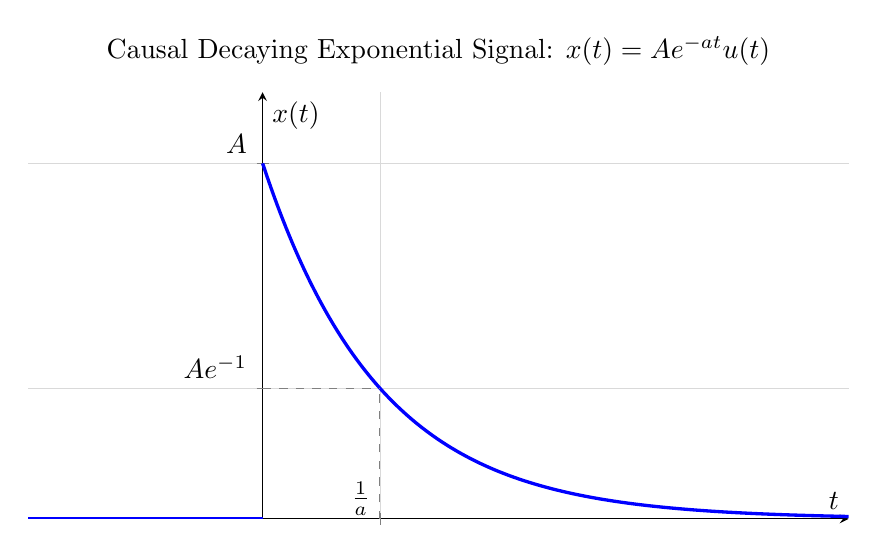
\begin{tikzpicture}
	\begin{axis}[
		width=12cm,
		height=7cm,
		xlabel={$t$},
		ylabel={$x(t)$},
		title={Causal Decaying Exponential Signal: $x(t) = A e^{-at} u(t)$},
		xmin=-2, xmax=5, % Increased xmin to show more of t<0
		ymin=0, ymax=1.2,
		axis lines=middle,
		xtick=\empty,
		ytick=\empty,
		extra x ticks={1},
		extra x tick labels={$\frac{1}{a}$},
		extra y ticks={0.3678, 1},
		extra y tick labels={$Ae^{-1}$, $A$},
		extra tick style={
			ticklabel style={anchor=south east}
		},
		grid=both,
		grid style={line width=.1pt, draw=gray!30},
		samples=200,
		no marks,
		]
		
		% Explicitly draw the zero line for t < 0
		\draw[blue, very thick] (axis cs:-2,0) -- (axis cs:0,0);
		
		% Plot the exponential function for t >= 0
		% The domain is set from 0 to xmax
		\addplot[blue, very thick, domain=0:5] {exp(-x)};
		
		% Add dashed lines to highlight the point at the time constant
		\draw[dashed, gray] (axis cs:1,0) -- (axis cs:1, {exp(-1)});
		\draw[dashed, gray] (axis cs:0,{exp(-1)}) -- (axis cs:1,{exp(-1)});
		
		
	\end{axis}
\end{tikzpicture}